\section{Isothermal compressible flow - H process}
\label{sec:h_gas}

The subject of this chapter is the movement of gases in porous media. In contrast to groundwater hydraulics, gas flow is more
complicated because of its compressibility. Significant variations
in air density and viscosity can result also from temperature
fluctuations (so-called Klinkenberg effect). According to the
kinetic theory of gases, its viscosity should not depend on the
pressure. This is not necessarily the case for conditions
typically existing in natural gas reservoirs \cite{VoiLau:1985}. At a fixed
temperature, the viscosity of gas can vary by tens of percents as
the formation pressure changes by a few Mega Pascale. Another
problem concerns the evidence of turbulent flow which results in
additional friction effects. The present verificational study is constrained to isothermal gas flow, where
analytical solutions exist. Non-isothermal effects are considered in section \ref{sec:nonisothermal_gas_flow}.
%
Simulation of compressible flows in porous media is neccessary for different applications such as air movement in soils, gas production or \CO2 storage if carbondioxide is injected in a gaseous state.

%-------------------------------------------------------------------------
\subsection{Theory}
\label{sec:air_flow}

The theory of gas seepage was developed
first by \cite{Muskat:1937}, \cite{Leibenzon:1947}, and \cite{AraNum:1965}, who worked out a number of analytical approximations to
solve the nonlinear problem. To this end, a number of general
assumptions must be introduced, e.g. gravitational forces are
neglected, no phreatic surfaces are formed, and idealized material
properties must be assumed. The state of the compressible fluid
within a considered closed system may be isothermal (const.
temperature), adiabatic (const. heat content), or polytropic
(const. change of heat content).
%
The equation of gas flow in a porous medium can be derived from
the mass balance of fluid (gas) mass
%
\begin{equation}
\frac{\p n \rho}{\p t}
+
\nabla \cdot (\rho n \VelocityVector)
=
Q_\rho
\label{eqn:fluid_mass_1}
\end{equation}
%
where $\rho$ is gas density, $\VelocityVector$ is velocity
vector, $n$ is porosity and $Q_\rho$ is a fluid mass density source/sink term.
%
The equation of state for an ideal gas (\ref{eqn:ideal_gas_law})
represents its compressibility and expansivity due to pressure and
temperature changes, respectively.
%
\begin{equation}
\rho
=
\frac{p}{R_{\mbox{\small air}}T}
\label{eqn:ideal_gas_law}
\end{equation}
%
where $p$ is gas pressure, $R_{\mbox{\small air}}$ is the specific gas constant which is for
air is equal to $287\,J/(kg K)$ and $T$ is
temperature in Kelvin. Therefore, the ideal gas density at atmospheric
pressure and $T=293K$ is
%
\begin{equation}
\rho
=
\frac{101325 Pa}{287 J/(kg K)\,293 K}
=
1.20433\,\frac{kg}{m^3}
\end{equation}
%
For isothermal flow, i.e. $T=T_0$ we have
%
\begin{equation}
n \frac{\p p}{\p t}
+
\nabla \cdot (p n \VelocityVector)
=
R_{\mbox{\small air}} T_0 Q_\rho
\end{equation}
%
In addition with the momentum balance equation, which can be
expressed in form of an extended Darcy's law for non-linear flow.
%
\begin{equation}
n\VelocityVector
=
-\frac{\PermTensor}{\mu}
\nabla p
\label{eqn:darcy_gas}
\end{equation}
%
where $\PermTensor$ is permeability tensor, $\mu$
is fluid viscosity,
%
the gas mass balance equation reads as
%
\begin{equation}
n\frac{\p p}{\p t}
-
\nabla \cdot
(p\frac{\PermTensor}{\mu}\nabla p)
=
R_{\mbox{\small air}} T_0 Q_\rho
\end{equation}
%
which is a non-linear equation with respect to gas pressure $p$.

%-------------------------------------------------------------------------
\subsection{Examples}

Two test examples for isothermal gas flow are presented. The first test case is dealing with 1-D compressible flow in a porous media where an analytical solution exists for the steady state (sec. \ref{sec:flow_test}). The second example shows the advantages of object-orientation in finite element implementation (sec. \ref{sec:element_test}).

\subsubsection{Compressible flow test}
\label{sec:flow_test}

We consider a simple 1-D test example where gas is injected at constant pressure into the porous medium. The material
parameters are summarized in Tab. \ref{tab:air_heat_1d}.

\begin{table}[htb!]
\centering
\begin{tabular}{llll}
\hline\hline\noalign{\smallskip}
Property & Symbol & Value & Unit \\
\noalign{\smallskip}\hline\noalign{\smallskip}
Model length & $L$ & $100$ & $m$\\
Cross section area & $A$ & $1$  & $m^2$ \\
Porosity & $n$ & $0.35$  & $-$ \\
\hline
Permeability & $k$ & $2.7\times 10^{-11}$ & $m^2$\\
Gas dynamic viscosity & $\mu$ & $1.76\times 10^{-5}$ & $Pa\,s$\\
Initial condition & $p_I$ & $101325$ & $Pa$\\
Boundary conditions & $p_1, p_2$ & $101325, 3 \times 10^6$ & $Pa$\\
\hline
Time step & $\Delta t$ & $1,10,10^2,10^3,10^4$ & $s$\\
Space step & $\Delta x$ & $1$ & $m$\\
\noalign{\smallskip}\hline\hline
\end{tabular}
\caption{Model parameters}
\label{tab:air_heat_1d}
\end{table}

For isothermal flow with Dirichlet boundary conditions, i.e. $p(0,t)=p_1$ and
$p(100,t)=p_2$, there exists an analytical solution,
%
\begin{equation}
p(x)
=
\sqrt{(p_2^2-p_1^2)\frac{x}{x_2-x_1}+p_1^2}
\label{eqn:press_analytical}
\end{equation}
%
which is used for verification of the present numerical solution. 
%
Fig. \ref{fig:air_steady} shows the comparison of present numerical solution with analytical. Steady state is reached after about $1.0\times10^4~s$.

\begin{figure}[htb!]
\begin{center}
\includegraphics[scale=0.5]{H_GAS/figures/gas_flow_new.eps}
\end{center}
\caption{Comparison of analytical (circles) and numerical solutions}
\label{fig:air_steady}
\end{figure}

According to Darcy's law (\ref{eqn:darcy_gas}) the volumetric gas flux at reference conditions can be approximated as follows
%
\begin{equation}
Q_0
=
A
\frac{T_0}{T^* p_0}
\frac{k}{\mu}
\frac{(p_2^2-p_1^2)}{2(x_2-x_1)}
\label{eqn:press_analytical}
\end{equation}

\subsubsection*{Benchmark repository}
\begin{tabular}{|l|l|l|l|}
\hline
Problem type & Repository path & Files & Version \\
\hline
\verb H_GAS & \verb benchmarks\h_gas\gas_flow & \verb h_gas_line & 4.10.07 \\
\hline
\end{tabular}

%-------------------------------------------------------------------------
\subsubsection{Element test}
\label{sec:element_test}

This example is presented first of all for code verification of all
element types implemented, i.e. lines, triangles, quads,
tetrahedra, triangle prisms and hexahedra \cite{WanKol:2007}. We consider a
non-linear problem, flow of a compressible fluid through the porous
medium. In this case the hydraulic conductivity is pressure dependent.

The discretizations with different element types is shown in Fig.
\ref{fig:h_elements}. The initial gas pressure distribution is equal
to $1.01325\times10^5~Pa$, everywhere in the model domain. There are Dirichlet
boundary condition set at left $p^g(x=0m)$ = $9.5500\times10^4~Pa$, and right hand side $p^g(x=100m)$ = $1.01325\times10^5~Pa$, respectively, in order to
extract gas from the domain. The material parameters of the fluid
and the porous medium are given in Tab. \ref{tab:apl_h}.

\begin{figure}[htb!]
\center
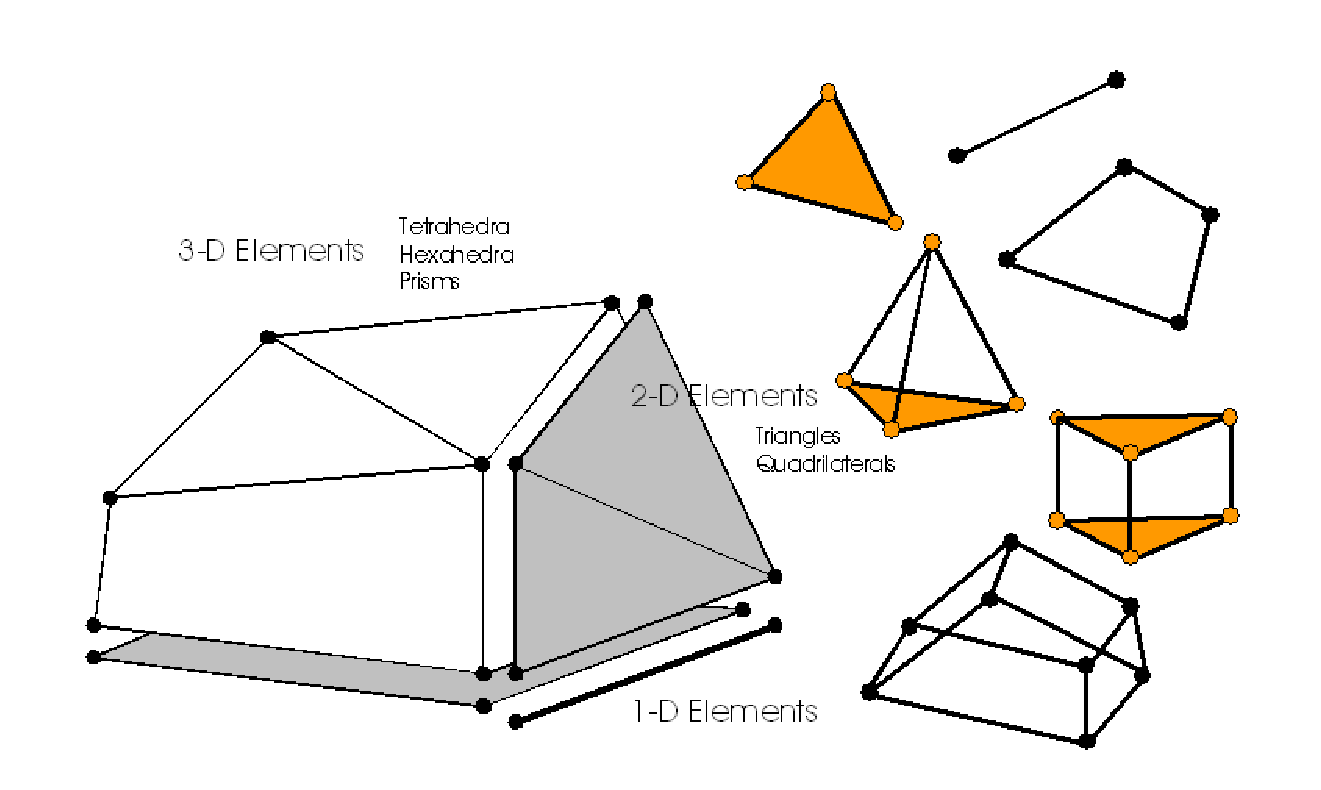
\includegraphics[scale=0.5]{H_GAS/figures/elements.eps}
\caption{Different element types} \label{fig:h_elements}
\end{figure}

\renewcommand{\baselinestretch}{0.9}
\begin{table}[htb!]
\centering
\begin{tabular}{llll}
\hline\hline
Property  &  Symbol & Value & Unit \\
\hline
Model length & $L$ & $0.05$ & $m$\\
Cross section area & $A$ & $1$  & $m^2$ \\
\hline
Viscosity & $\mu$ & 1.78$\times 10^{-5}$ & $Pa\,s$ \\
\hline
Porosity & $n$ & 0.005 & $-$\\
Permeability & $k$ &  2.77$\times 10^{-19}$ & $m^2$ \\
\hline
Time step & $\Delta t$ & $ 3\times 10^2$ & $s$\\
Space step & $\Delta x$ & $0.005$ & $m$\\
\hline\hline
\end{tabular}
\caption{Material parameters}
\label{tab:apl_h}
\end{table}

Fig. \ref{fig:gas_flow} depicts the temporal evolution of gas
pressure at the observation point at the outlet. The numerical
results of all implemented element types compare very well. Small
deviation occur from different numbers of Gauss integration
points.

\begin{figure}[htb!]
\center
\includegraphics[scale=0.5]{H_GAS/figures/gas_flow.eps}
\caption{Evolution of gas pressure at the outlet observation point}
\label{fig:gas_flow}
\end{figure}

\subsubsection*{Benchmark repository}
\begin{tabular}{|l|l|l|l|}
\hline
Problem type & Repository path & Files & Version \\
\hline
\verb H_GAS & \verb benchmarks\h_gas\element_test & \verb h_gas_* & 4.10.07 \\
\hline
\end{tabular}

